% !TeX spellcheck = en_US
\newpage
\section{Infrastructure security}
There are different security \textbf{objectives}:
\begin{itemize}
	\item \textbf{Confidentiality}: to ensue nondisclosure of data
	\item \textbf{Integrity}: to ensure completeness and accuracy of data
	\item \textbf{Authenticity}: to allow for the verification of identity
\end{itemize}

\subsection{Cryptography}
Many security goals may be achieved through \textbf{cryptography}.
\begin{center}
	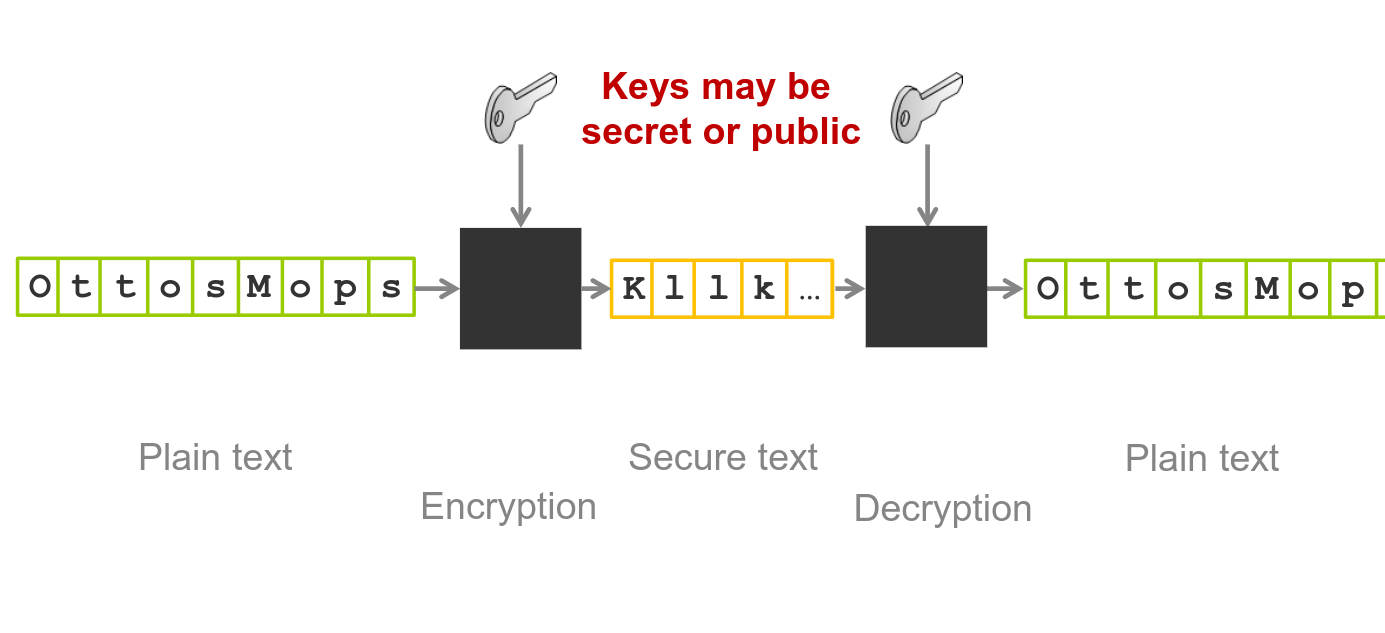
\includegraphics[scale=.25]{crypto}
\end{center}	
There are two types of cryptography:
\begin{itemize}
	\item \textbf{Symmetric}: the same key, which remains always private, is used for encryption and decryption
	\item \textbf{Asymmetric}: different keys are used for encryption and decryption, \textbf{private} and \textbf{public}
\end{itemize}

\begin{table}[!h]
	\centering
	\begin{tabular}{c|c|c}
		& \textbf{Public key} & \textbf{Private key} \\
		\hline
		\textbf{Confidentiality} & Encryption & Decryption \\
		\textbf{Authenticity} & Decryption & Encryption
	\end{tabular}
\end{table}
\subsubsection{Trust}
The main challenge in the public/private key context is to obtain \textbf{trust} in the public key. A \textbf{Public Key Infrastructure} manages that a \textit{public key} belongs to entities such as persons or organizations. If you trust the PKI, then you trust the key itself.\\
A \textbf{certificate authority} signs the public key of a third party by its own private key, attesting that the first one is correct. If you trust the CA, you also trust the third party key.

\subsection{DNSSEC}
DNS main problems are:
\begin{itemize}
	\item DNS resolver can \textbf{lie} about DNS answer
	\item DNS client cannot verify the correctness of the answer
\end{itemize}
The objectives of DNSSEC are to provide \textbf{integrity} to prevent \textit{spoofing} and \textit{poisoning}. That is done through;
\begin{itemize}
	\item \textbf{Authenticating messages} of name servers: check that no one on the way changed the DNS content
	\item \textbf{Authenticating resources records}: check that data comes originally from authoritative DNS servers
	\item \textbf{Proof of non-existence}: prevent DoS against names
\end{itemize}
DNSSEC is based on private key cryptography and introduces new resource records:
\begin{itemize}
	\item \textbf{RSIG}: contains cryptographic signature
	\item \textbf{DNSKEY}: contains public sign key
	\item \textbf{DS}: contains hash of the \textit{DNSKEY}
	\item \textbf{NSEC/NSEC/3}: for explicit denial-of-existence of  DNS records
	\item \textbf{CDNSKEY/CDS}: for a child zone requesting updates to DNS records in the parent zones
\end{itemize}
The main objectives of DNSSEC are:
\begin{itemize}
	\item \textbf{Secure a zone}: DNSSEC does not sign resource records individually but signs \textbf{Resource Record Sets}. It distinguishes between two types of pair:
	\begin{itemize}
		\item \textbf{Zone}-Signing-Key: it starts with a \textbf{root zone key}, the highest possible in the DNS tree, and then follows cryptographic pointers to lower zones. Each pointer is validated with the previous validated \textbf{zone key}. This is called a \textbf{chain of trust} and works so that a resolver has only to carry the root key to validate the DNSSEC data on the Internet.
		\item \textbf{Key}-Signing-Key: it operates the same as ZSK: signs the ZSK and stores it in DNSKEY and creates RRSIG for it
	\end{itemize}
	\item \textbf{Secure zone delegation}
\end{itemize}

\begin{observation}
	Deployment usually work two ways:
	\begin{itemize}
		\item \textbf{Full DNSSEC}: it's DNSSEC compliant and performs validation on its own
		\item \textbf{Stub resolver}: usually deployed on end hosts to perform DNS queries
		\begin{enumerate}
			\item Client trusts completely the server
			\item Client decides autonomously how to handle unauthenticated data, either by enforcing validation or less
		\end{enumerate}
	\end{itemize}
\end{observation}

\subsection{RPKI}
Exploiting BGP Updates could lead to traffic \textbf{interception} to break privacy or service availability, since it's based on trust. Any BGP speaker can claim to own an IP prefix or modify an AS path. A receiver cannot verify the correctness of these data. \\\\
There are three threats models for the BGP protocols:
\begin{itemize}
	\item \textbf{Route leaks}
	\item \textbf{AS Path manipulation}: change the AS path compared to the original traversal. The solution is to map IP prefixes to origin AS necessarily, including \textbf{cryptographic proof} so that prefix owner can authenticate it.
	\item \textbf{Prefix Origin Hijacking}: originate an IP prefix that you don't own. The solution is to sign paths so that BGP path information are cryptographically secured
\end{itemize}

\textbf{Resource Public Key Infrastructure} is a system that allows to attest the usage of IP addresses and internet resources, and thus includes cryptographically provable certificates that reflect IP/AS allocation in the Internet. Currently each RIR creates a self-signed root certificate.

\subsection{ROA}
A \textbf{Routing Origination Authority} legitimates an AS to originate IP addresses. It contains:
\begin{itemize}
	\item Set of IP prefixes with minimal and maximal (optional) length
	\item An AS number allowed to announce the prefixes
	\item End-Entity-Certificate
\end{itemize}
They will be signed with the certificate of a RPKI